\documentclass[a4paper,oneside,10pt,titlepage]{article}

\usepackage[utf8]{inputenc}
\usepackage{a4wide}
\usepackage{lmodern}
\usepackage{graphicx}
\usepackage{amsmath}
\usepackage{amsfonts}
\usepackage{tikz}
%\usepackage{eurosym}
\renewcommand*{\familydefault}{\sfdefault}
\renewcommand{\contentsname}{Inhaltsverzeichnis}

\begin{document}
\linespread{.9}
\pagestyle{empty}
\title{Personalisierbare\\Datenverarbeitung und Visualisierung\\von Wetterprognosedaten}
\author{\\\\\\\\\\\\\\\\\\\\\\Markus Becker\\Swenja Wagner}

\maketitle
\pagestyle{empty}
\tableofcontents
\thispagestyle{empty}
\pagestyle{plain}
\newpage

\begin{abstract}
abstract
\end{abstract}

\section{Auvi}
\begin{center}
\scalebox{0.56}{
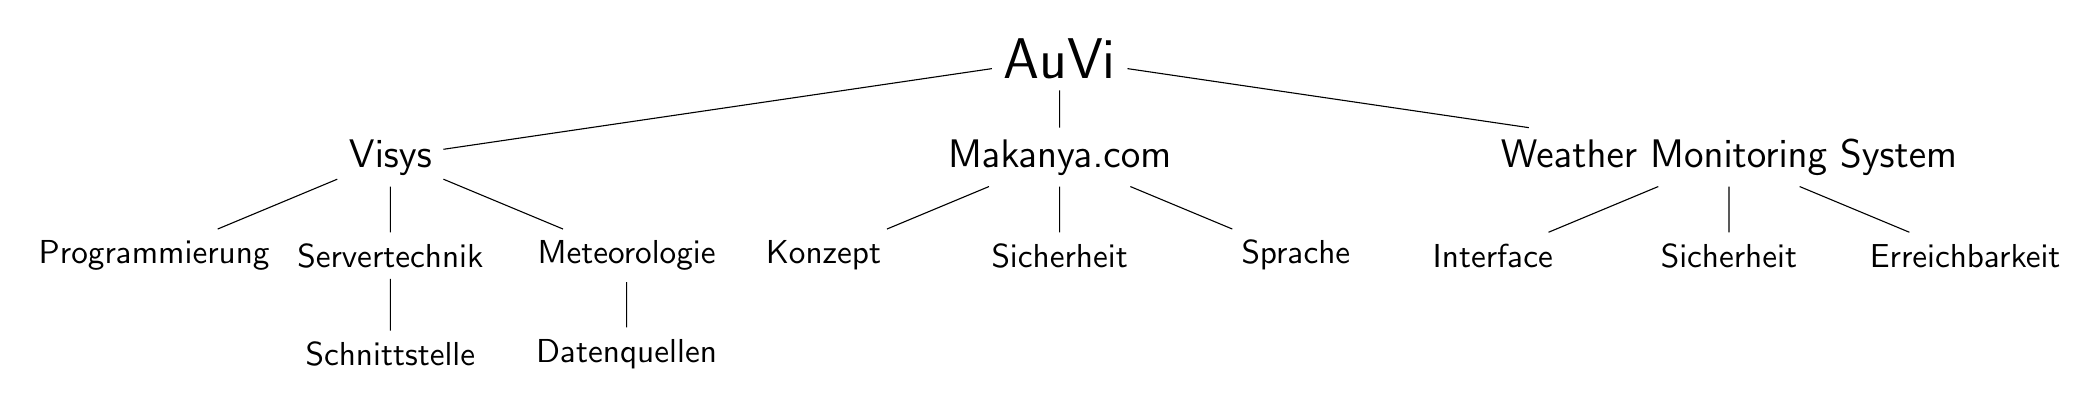
\begin{tikzpicture}[
every node/.style = {scale=1.2},
level 1/.style = {sibling distance = 8.5cm},
level 2/.style = {sibling distance = 3cm},
level 3/.style = {sibling distance = .5cm},
level distance = 1.25cm
]
\node {\LARGE AuVi}
	child { node {\large Visys} 
		child { node {Programmierung}}
		child { node {Servertechnik}
			child { node {Schnittstelle}}		
		}
		child { node {Meteorologie}
			child { node {Datenquellen}}		
		}
	}
	child { node {\large Makanya.com} 
		child { node {Konzept}}
		child { node {Sicherheit}}
		child { node {Sprache}} 	
	}
	child { node {\large Weather Monitoring System} 
		child {node {Interface}}
		child {node {Sicherheit}}
		child {node {Erreichbarkeit}}
	};
\end{tikzpicture}
}
\end{center}
\subsection{Programm}
eine allgemeine Erklärung, was das Programm kann, damit der Leser sich zurecht findet

\subsection{Meteorologie}
\subsubsection{Prognosetheorie}
Was ist eine Prognose in der Meteorologie?
Die Meteorologie gehört zu den Naturwissenschaften. Sie liefert die Voraussetzungen um eine Wettervorhersage erstellen zu können. Unter einer Wetterprognose versteht man die Vorhersage eines Zustands der Atmosphäre zu einem bestimmten Zeitpunkt an einem bestimmten Ort oder in einem bestimmten Gebiet. Es wird nicht nur das Wetter in Bodennähe betrachtet, sondern auch Wettererscheinungen in höheren Erdatmosphären.
\\
Das Wetter lässt sich durch entsprechende Naturgesetze beschreiben. Das ist für die Prognose essentiell wichtig. Der Grundgedanke einer solchen Prognose besteht darin, aus einem bereits vergangenen und dem aktuellen Zustand der Atmosphäre einen Zustand in der Zukunft abzuleiten. Dazu werden die bekannten physikalischen Regeln angewendet. In mathematischer Hinsicht werden diese physikalischen Regeln von nichtlinearen Gleichungen beschrieben. Das bedeutet, dass bereits die kleinste Änderung im Ausgangszustand das Ergebnis der Rechnung relativ groß verändern kann.%[1]
\subsubsection{Prognosen per Hand}
Was muss man über die aktuelle Situation wissen um per Hand eine Prognose zu erzeugen?
Es gibt einen Unterschied zwischen der manuellen oder auch synoptischen Wettervorhersage und einer numerischen Wettervorhersage. In der synoptischen Meteorologie ist ein System aus Beobachtungsstationen nötig, die gleichzeitig Wetterbeobachtungen nach einem einheitlichen Verfahren durchführen. Die Stationen messen unter anderem Parameter wie: Luftdruck, Luftdruckänderung während der letzten drei Stunden, Lufttemperatur, Windrichtung, Windgeschwindigkeit, Taupunkt, Wolkenart, Höhe der Wolkenuntergrenze, Bedeckungsgrad, Sichtweite, Niederschlagsmenge und Niederschlagsart. Es wird zwischen Bodenbeobachtungsstationen, die Daten in der Nähe der Bodenoberfläche sammeln und aerologischen Beobachtungsstationen, die Daten aus bis zu 30km Höhe liefern unterschieden. Es werden auch Daten von mobilen Messstationen, wie Bojen und Flugzeugen verwendet. Wettersatelliten und Fernerkundungssystem (wie Wetterradar, Blitzortungssysteme, LIDAR, SODAR) könne auch als Datenquelle dienen. Die gesammelten Daten, die den Wetterzustand zu einem bestimmten Zeitpunkt beschreiben, werden in Wetterkarten eingetragen. (zum Beispiel Bodenwetterkarten) Mit Hilfe der eingetragenen Daten werden die Wetterverhältnisse analysiert und Wettervorhersagen erstellt. Zusätzlich dazu werden die gesammelten Daten von numerischen Vorhersagemodellen als Ausgangszustand verwendet. %[2]
\\
Numerische Wettervorhersagen sind rechnergestützt. Der Zustand der Atmosphäre zu einem späteren Zeitpunkt wird aus dem Zustand der Atmosphäre zu einem gegebenen Anfangszeitpunkt berechnet. Dabei werden relevante GLeichungen numerisch gelöst (Navier-Stokes-Gleichung, thermische Zustandsgleichung idealer Gase, erster Hauptsatz der Thermodynamik, Kontinuitätsgleichung). Bei solchen numerischen Vorhersagemodellen wird das betrachtete Gebiet in Gitterzellen unterteilt. Für jeden Bereich werden dann die Parameter errechnet. Relevante physikalische Größen sind vor allem Temperatur, Luftdruck, Dichte, Windrichtung und Windgeschwindigkeit. Es wird zwischen Globalmodellen und Lokal- oder Ausschnittsmodellen unterschieden. Aufgrund des großen Aufwands die Daten zu errechnen, werden Supercomputer verwendet.
\subsubsection{Voraussetzung für Datenprognosen}

\subsection{Datenquellen}
\subsubsection{Quellenvergleich}
Da wir nun dargestellt haben, dass es für uns nicht möglich ist unsere eigenen Daten zu generieren, zeigen wir nun welche Quellen die benötigten Daten zur Verfügung stellen. Der Nutzer kann selbst zwischen den verschiedenen Datenquellen wählen, die angeboten werden. Die angebotenen Datenquellen können über die GUI gewählt werden.

Wir werden über eine GUI (graphic user interface) dem Nutzer anbieten zwischen verschiedenen Datenquellen zu wählen. Diese werden wir auch statistisch vergleichen.
Grafik: Übersicht über Quellen (Alle die direkt über das Programm angeboten werden)
Programm kann um weitere erweitert werden.
Auswahl NOAA, GFS.
\subsubsection*{Wetterdienst}
Wir geben an was der DWD bietet und wie viel er kostet.
Grafik: Diagramm der Genauigkeit
\subsubsection*{NOAA Global Forecast System}
Wir geben an was das GFS bietet und warum wir es als Hauptdatenquelle verwenden.
Grafik: Diagramm der Genauigkeit

Das Global Forecast System (GFS) ist ein Modell, das mathematisch Parameter errechnet.Es ist also ein numerisches Vorhersagemodell. Die dazu benötigten Daten bezieht es aus einem Netz von Wetterstationen, die sowohl an Land als auch im Wasser und in der Luft Messungen durchführen. Mit diesen gemessenen Daten werden mithilfe von geophysikalischen Gesetzen weitere Daten errechnet. So wird in einem Abstand von 13,5km je ein Wert ermittelt. Diese Daten werden als große Datensätze kostenfrei auf der Webseite ()  zur Verfügung gestellt.
\subsubsection{Datenverfügbarkeit}
Wie weit in die Zukunft können die Quellen schauen. Wodurch sind sie begrenzt, Wie oft muss man die Daten generieren und abrufen?
Grafik: Diagramm der Zukunftsdaten
\subsection{Entwicklung}
\subsubsection{Wahl der Umgebung}
sofware und hardware
\subsubsection{Methodik}
wer wann wie wo
\subsubsection{genutzte Mittel}
website, server, ...
\subsubsection{Servertechnik}
Beschreibung Architektur, Ordnerstruktur
\subsection{Schnittstelle mit dem Nutzer}
\subsubsection{Webseite}
\subsubsection{Datenformate}
html, php, png, jpg
\subsubsection{Schulhompage}
\subsection{Szenario}
Wir werden nun Beispiele angeben, wie unser Programm genutzt werden kann. Es gibt darüber hinaus unendlich viele Möglichkeiten aus dem Programm individuellen Nutzen zu ziehen.
\subsubsection{Frühwarnung}
% Nach dem Ampel System eigene Parameter die Gefährdung darstellen markieren. Z.B. Segler mit Windgeschwindigkeit auf Seelevel, Segelflieger mit Windgeschwindigkeit und Richtung auf x-Meter Höhe. Allgemeiner Arbeiter mit Temperatur.
Das von uns entwickelte System kann verwendet werden um wetterbedingte Gefahrensituationen frühzeitig zu erkennen. Anhand der globalen Datenquellen und dem Hintergrund unseres Systems ist es einem Nutzer möglich für seinen Ort selbst die Parameter zu wählen die für Ihn eine Gefährdung darstellen.\\
Es ist uns wichtig, dass unsere Visualisierung keine Laien abschreckt, deshalb haben wir uns entschieden die Frühwarnung in Form eines Ampelsystems an den Nutzer zu bringen. Dieser kann bei Interesse an der Frühwarnfunktionalität eine Spanne angeben, in der der entsprechende Parameter sicher ist (grün), gefährlich wird (gelb) oder gefährlich ist (rot). Diese sehr visuelle Form soll dabei auf einem Blick ermöglichen die Wetterlage abzuschätzen.\\
Für detailierte Auswertungen bieten wir andere Anzeigeformate an.
\subsubsection{Exotische Orte}
Ob mitten im Ozean oder in der Wüste, unser Programm liefert Prognosen für jeden Ort. Wir benötigen nur die dazugehörigen Koordinaten. Die Genauigkeit ist von der Zeitspanne und der Entfernung zur physikalischen Messstation abhängig. Je weiter das Wettereireignis in der Zukunft liegt, desto geringer ist die Genauigkeit. Die Genauigkeit steigt, wenn sich eine Messstation im näheren Umfeld befindet.
\subsubsection{Wissenschaft}
Wissenschaftler können von uns bereitgestellte Parameter kombinieren und sich so neben allgemein komplexeren meteorologischen Daten auch besonders interessante meteorologische Ereignisse grafisch darstellen lassen. Wenn jemand zum Beispiel Zusammenhänge zwischen der Ozonschicht und der Temperatur erforscht, kann er sich eine Grafik ausgeben lasse, die ihm diese beiden Parameter darstellt.
% Dr. Eixmann fragen, was man sich wissenschaftlich visualisieren könnte
Grafik: Ozon/Temperatur o.ä.
\subsubsection{Anpassung}
Wie zuvor genannt kann der Nutzer eigene Muster einstellen und so das Programm erweitern.
Grafik: Tabelle im Programm, Text als Datei.
% Inhalte für die besondere Lerleistung
\subsection{Öffentlichkeitsarbeit}
Messen, Vorträge, Dokumentation, Poster
Um unsere Arbeit zu präsentieren, entstanden im Laufe des Projekts mehrere Poster. Anfangs designten wir diese in Power Point, sind dann allerdings auf Gimp umgestiegen, da sich das für unsere Arbeit vorteilhafter gestaltete. Auf den Postern war meist zuerst eine kleine Einführung in das Projekt. Danach schloß sich eine nähere Erläuterungen desselben an. Um das Poster für den Betrachter attraktiver und anschaulicher zu machen, stellten wir einige Themen in grafischer Form dar und veranschaulichten unsere Ergebnisse mit Beispielgrafiken. \\
Häufig wurde auch eine schriftliche Erläuterung des Projekts gefordert, in der alles ausführlich erklärt wird. Diese Dokumentation des Projekts schrieben wir in LateX. Auch in diesen Dokumentationen wurden Übersichten und Grafiken als Anschauungsmaterial beigefügt und nötigenfalls näher erläutert.\\
Solche Dokumentationen und Poster kamen zum Beispiel bei den Landeswettbewerben Jugend Forscht in Rostock (Mecklenburg Vorpommern) zur Anwendung. Bei diesem Wettbewerb werden aus dem gesamten Bundesland Projekte aus verschiedenen Fachgebieten präsentiert. Es wird unteteilt in Arbeitswelt, Biologie, Chemie, Mathematik/Informatik, Geo- und Raumwissenschaften und Technik. Die jeweils Erstplatzierten in jedem Bereich qualifizieren sich für den darauffolgenden Bundeswettbewerb. Am Landeswettbewerb nahmen wir erstmalig 2013 teil. Allerdings hatten wir uns erst kurz vorher zusammengefunden, sodass wir das Projekt unserer Vorgänger vorstellten. Wir nahmen am Wettbewerb teil um erste Erfahrungen zu sammeln und uns darüber klar zu werden, wo wir einmal hin wollen. Im darauf folgenden Jahr erreichten wir mit unserem Projekt "Auvi - Automatisierte Visualisierung von Wetterstations- und Wetterprognosedaten" den zweiten Platz in der Kategorie Geo- und Raumwissenschaften. Wir arbeiteten weiter an unserem Projekt und im Jahr 2015 gewannen wir den Landeswettbewerb sogar mit dem Projekt "AuVi - Automatisierte Visualisierung von meteorologischen Daten" und qualifizierten uns so für den Bundeswettbewerb.\\
Wir nahmen auch an weiteren Veranstaltungen teil, bei denen wir unser Projekt vorstellten. Dazu gehört zum Beispiel der IHK-Schulpreis. Im Jahr 2014 bewarb sich unsere Schule mit dem Projekt CampusPro. Wir durften zusammen mit Vertretern aus anderen Projekten unsere Schule bei dieser Veranstaltung vertreten. Im Jahr darauf nahmen wir wieder daran teil. Diesmal allerdings mit unserem Projekt an sich.\\ An unserer Schule wird die Möglichkeit geboten durch umfassende Projektarbeit ein IHK-Zertifikat zu erlangen. Um dieses zu erlangen werden Vorträge gehalten, in denen das jeweilige Projekt präsentiert wird. Im Jahr 2014 eröffneten wir solch eine Vortragsveranstaltung, indem wir kurz unser neues Projekt vorstellten. Im Jahr 2016 werden wir uns dann selbst um ein IHK-Zertifikat bemühen.
\section{Weather Monitoring System}
% wms.viwetter.de
% Was ist WMS BEGIN
Das Weather Monitoring System (kurz WMS) beschreibt eine Reihe von Bildschirmen die verteilt in Kühlungsborn Grafiken eines zentralen Servers anzeigen sollen. Diese Grafiken enthalten generelle Informationen über Kühlungsborn, sowie Wetterdaten und Wetterprognosen. Im Schulzentrum Kühlungsborn findet man eine weitere Anwendung des WMS. Das Foyer.
% Was ist WMS ENDE
\subsection{Konzept}
% Was war unsere Aufgabe
Schüler sollen in der Lage sein die von ihnen in der Projektarbeit erzeugten Grafiken über ein möglichst einfaches Interface auf einen Server zu laden. Sie sollen anschließend die Bilder ersetzen bzw. löschen können. Damit die Serveradministrator, in diesem Fall Swenja Wagner, Markus Becker und Dr. Eixmann, bestimmen können wer für welchen Ordner Grafiken hochladen und einbetten kann ist der Zugriff auf die Dateimanagementfunktion nur über ein Benutzerkonto möglich. Es können von jedem Administrator nach Bedarf neue Konten erstellt werden.
\subsection{Interface}
Nachdem ein Nutzer die Einlogroutine durchgeführt hat wird ihm die Struktur der Daten nach Anzeigeindex geordnet angezeigt.
\subsection{Erreichbarkeit}
\subsection{Sicherheit}
Da dieses System an öffentlichen Orten Anwendung finden soll, muss gewährleistet sein, dass auf den Anzeigegeräten nur Daten eingezeigt werden, die von autorisierten Personen ausgewählt worden. Außerdem soll der Service nicht ohne unsere Erlaubnis und Wissen aufrufbar sein, deshalb haben wir ein Accountsystem inplementiert. Da die Clientpc's automatisiert starten sollen und gleich die richtigen Daten anzeigen sollen, mussten wir ein Protokoll entwickeln, welches sicher ist, aber einem Rechner ermöglicht sich selbst einzuloggen.

\section{Makanya}
\subsection{Hintergrund}
Kooperation mit Kirchengemeinde, Schule, Tansania
\subsection{Methodik}
\subsection{Ergebnis}

\newpage
\Large{Selbstständigkeitserklärung}\\
\\
\small Hiermit erklären wir, dass wir die vorliegende Arbeit selbständig angefertigt, nicht anderweitig zu Prüfungszwecken vorgelegt und keine anderen, als die angegebenen Hilfsmittel verwendet haben. Zudem waren alle verwiesenen Webseiten zum Zeitpunkt der Linksetzung gültig und erreichbar. Wörtlich und sinngemäße Übernahmen aus anderen Werken sind als solche gekennzeichnet.
\\



\end{document}